\section{Introduction}
\label{sec:intro}

\begin{figure}[t]
\centering
  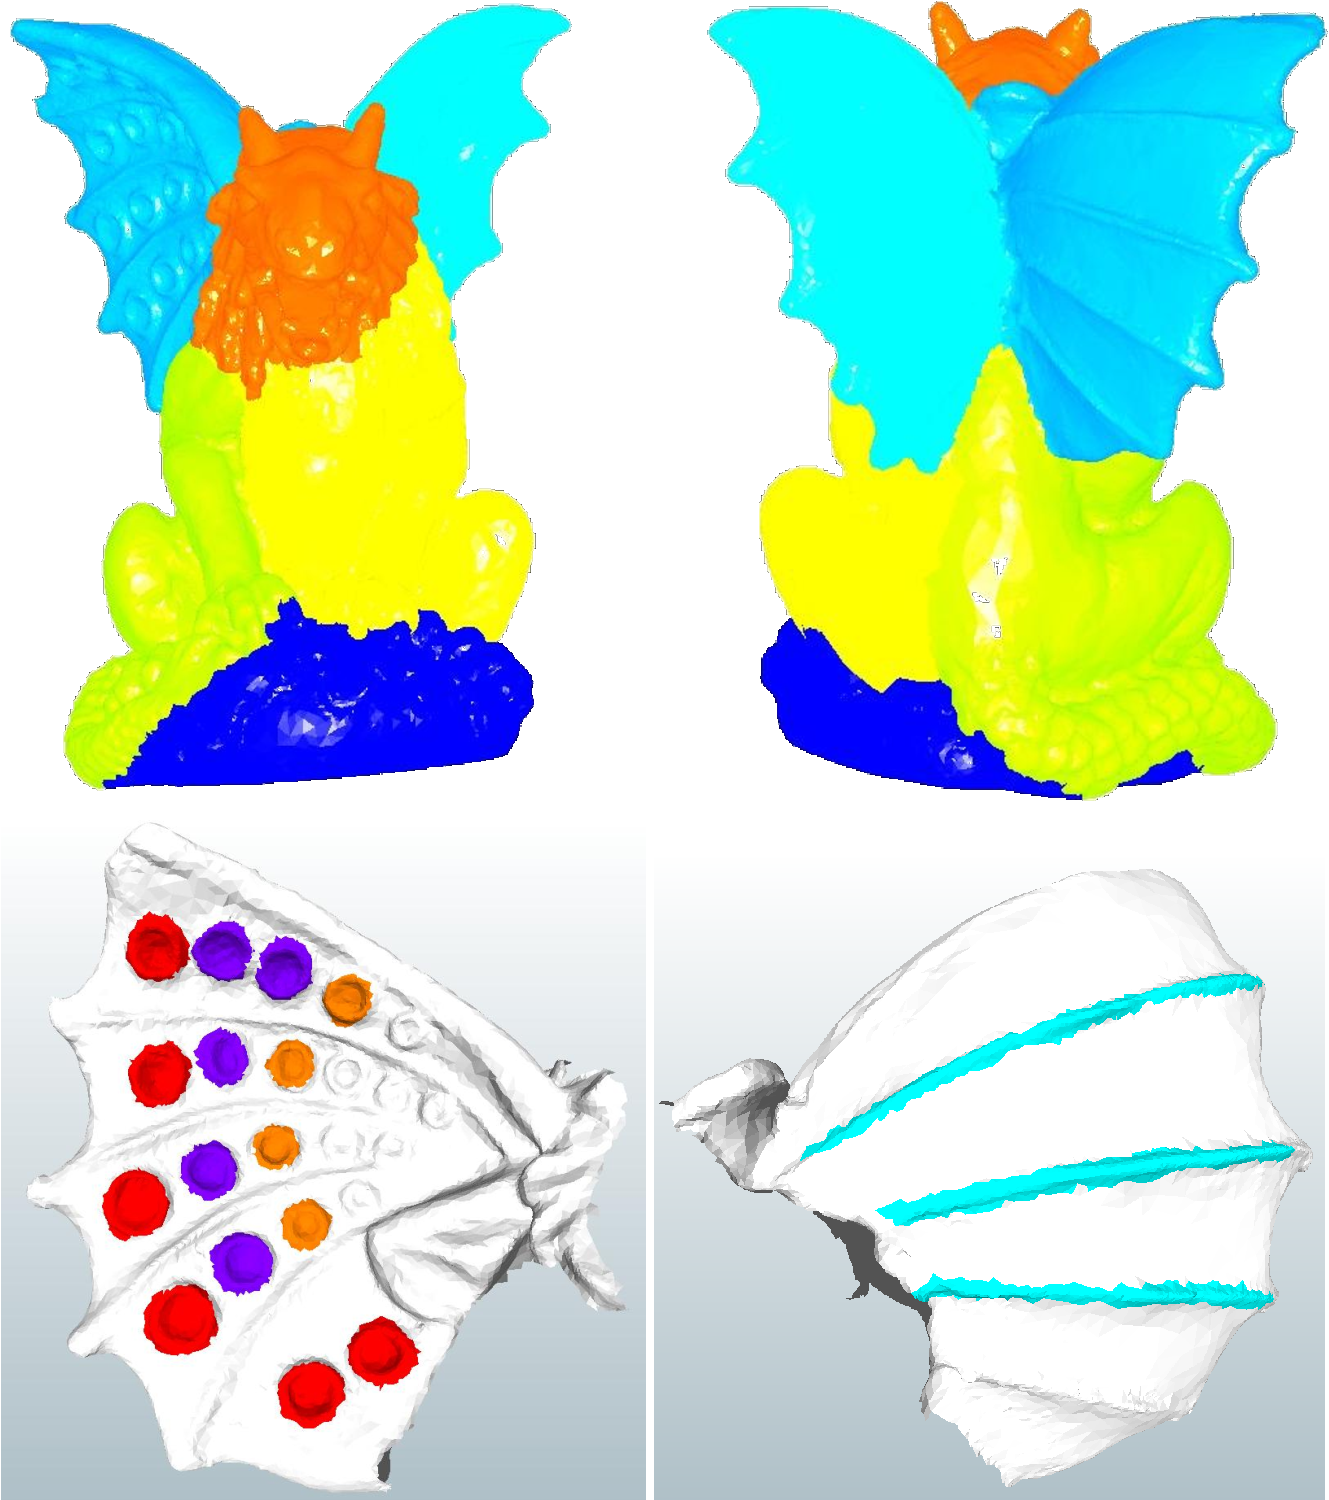
\includegraphics[width=0.99\linewidth]{figures/Gargoyl.pdf}
  \caption{Two-scale symmetries of the Gargoyle statue from two viewpoints.
  Top: At the coarse scale, two pairs of mirroring symmetry from six segmented parts are represented, with each pair being rendered by the same color.
  Bottom: At the fine scale, translation and rotation symmetries are detected on the left wing part for the detailed rings.}
\label{fig:Gargoyl}
\end{figure}

Many objects, both man-made and natural, have some symmetries or self-similarities in them.
Finding the symmetry from triangle shapes is a way to augment shapes with some structures thus helps various applications such as remeshing~\cite{podolak2006}, shape simplification~\cite{pauly2008},
segmentation~\cite{Shamir2008,mitra2006,xu2009}, repairing~\cite{bokeloh2009,berner2011}, and reconstruction~\cite{zabrodsky1997}.
Symmetry detection and analysis is a fundamental technique in computer graphics, computer vision and geometry processing.

Symmetries may have different definitions. In this work, we focus on generalized partial symmetry~\cite{mitra2006,berner2011} where some subsets of a shape reoccur multiple times within the model differing by combinations of translation, rotation and/or mirroring. Intrinsic symmetries are also considered in which case further isometric deformation is allowed between copies. This flexible definition allows symmetry detection to be more useful.

Whilst a lot of attention has been received in recent years, it still not clearly address the relationship between segmentation and symmetry detection.
Existing work mainly uses the symmetry detection to segment the shape, as symmetry has more semantic information than the segmentation.
But, the inverse problem, i.e. segmentation-based symmetry detection, has been almost not investigated until now.  
As we surveyed, all symmetry detection algorithms explicitly or implicitly used one rule, that is the symmetry subregion of the shape is the meaningful part.
This is also the foundation of the paper, but we employ the segmentation results to benefit symmetry detection.
The segmentation and symmetry detection could be further iteratively performed to produce more reasonable results.

In this paper, we propose an effective method for generalized partial symmetry detection.
The input shape is first segmented into multiple meaningful pieces. The correspondence between every pair of pieces
is established using robust matching.
This is followed by a clustering stage where consistent matchings are recognized as a symmetric pair.

Compared to the recent graph matching algorithms~\cite{bokeloh2009,berner2011} based on salient lines, our algorithm could produce more robust partial symmetry detection results.
As shown in Figure~\ref{fig:Gargoyl}, which is a failure case in~\cite{berner2011}, the two-scale symmetries of the Gargoyle statue are correctly detected.
The top row shows the coarse-scale mirroring symmetry detected from six meaningfully segmented parts (head, left and right wing, left and right body parts, and status base).
Two pairs of mirroring symmetries (shaded in the similar color) have been found.
The bottom row shows the fine-scale symmetry detection on the left wing, both the translational and rotational symmetries have been found for the detailed rings.

The rest of the paper is structured as follows. After surveying related previous work in Section 2, Section 3 describes our symmetry detection algorithm.
Section 4 demonstrates the effectiveness of our method with some results and comparisons with related works. Finally, section 5 draws conclusions and gives some discussions about future directions. 